%%导言区
\documentclass{ctexart}%ctexbook, ctexrep

% 导言区: \usepackage{graphicx}
% 语法: \includegraphics[< 选项 >]{< 文件名 >}
% 格式:EPS,PDF,PNG,JPEG,BMP
\usepackage{graphics}
\graphicspath{{figures/},{/pictures}} %图片在当前目录下的figures目录

% 正文区(文稿区)
\begin{document}
	\LaTeX{}中的插图:
	
	
\includegraphics{lion.eps}
	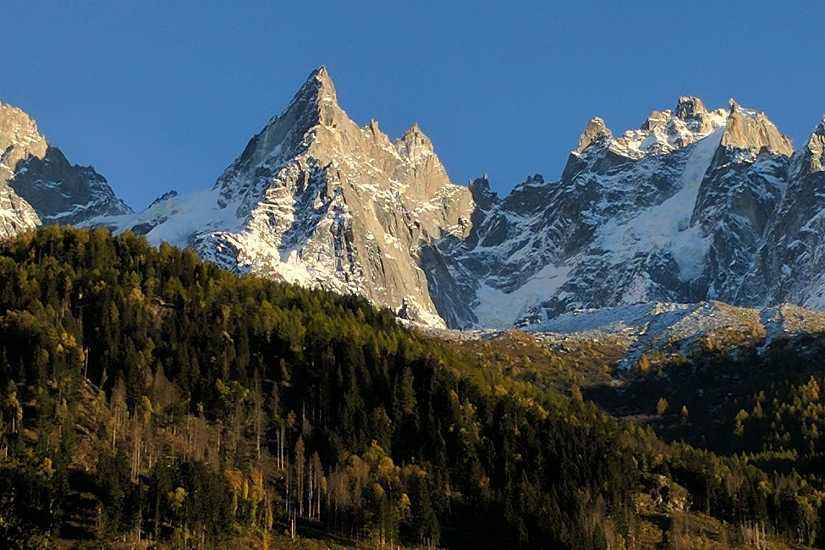
\includegraphics{mountain.jpg}
	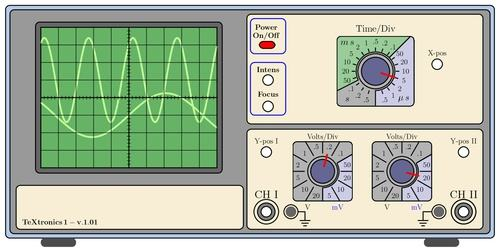
\includegraphics{oscilloscope.pdf}
	
	
\includegraphics[scale=0.3]{lion}
	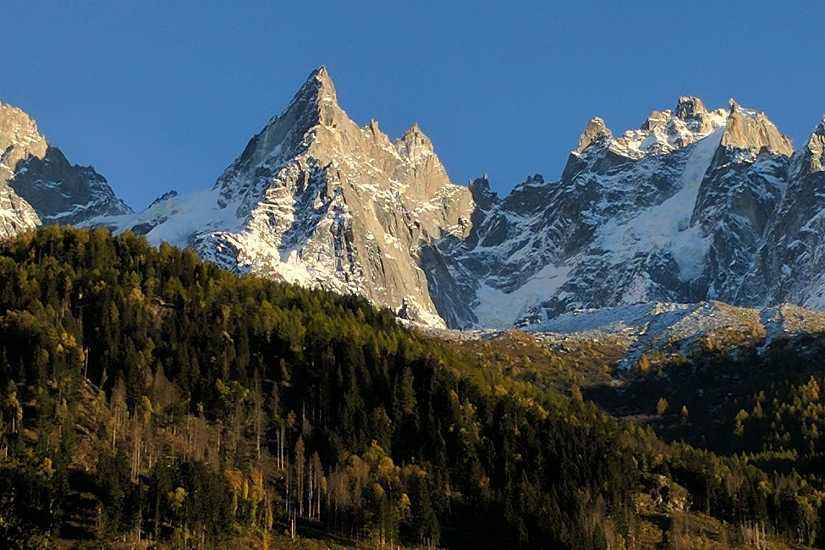
\includegraphics[scale=0.03]{mountain}
	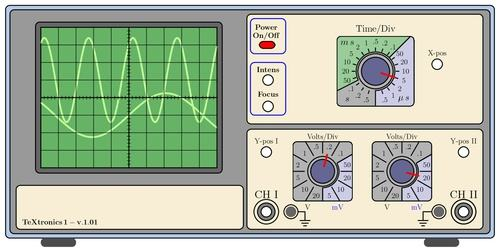
\includegraphics[scale=0.3]{oscilloscope}
	
	
\includegraphics[height=2cm]{lion}
	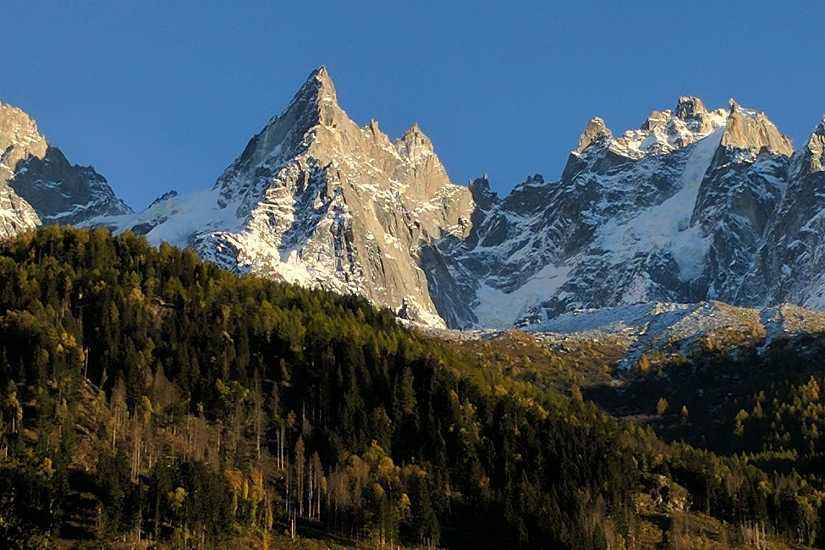
\includegraphics[height=2cm]{mountain}
	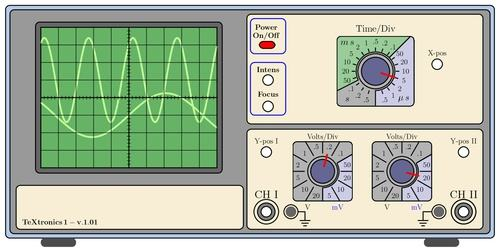
\includegraphics[height=2cm]{oscilloscope}
	
	
\includegraphics[width=2cm]{lion}
	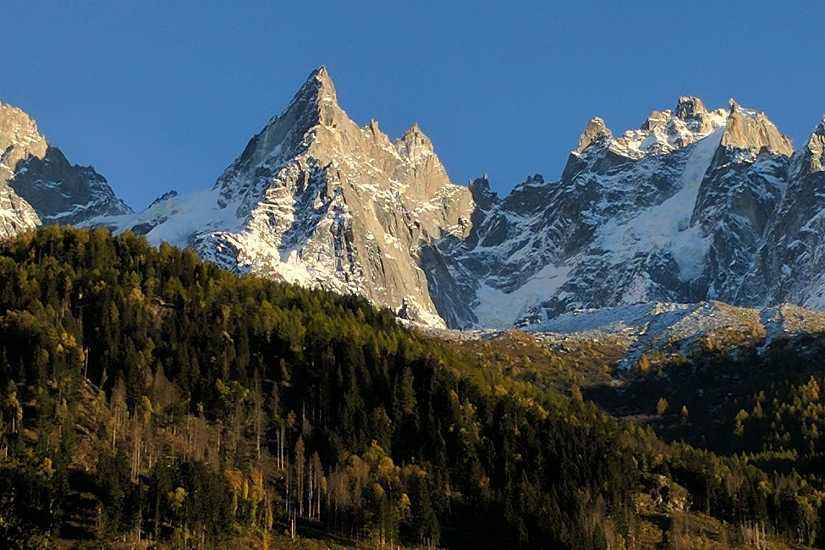
\includegraphics[width=2cm]{mountain}
	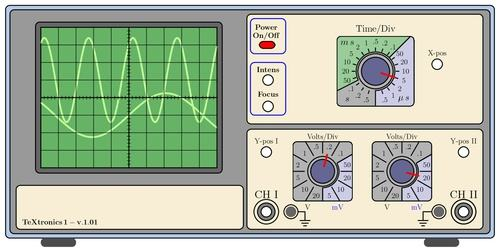
\includegraphics[width=2cm]{oscilloscope}	
	
	
\includegraphics[height=0.1\textheight]{lion}
	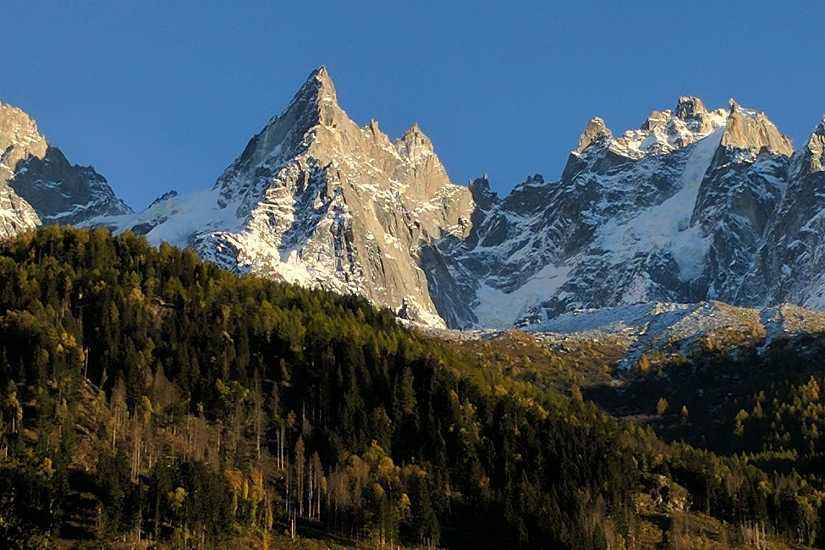
\includegraphics[height=0.1\textheight]{mountain}
	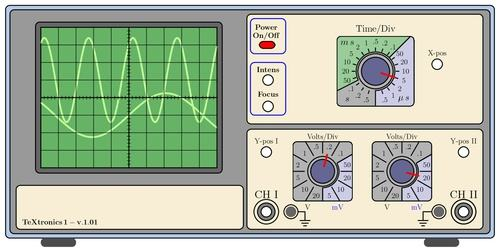
\includegraphics[height=0.1\textheight]{oscilloscope}
	
	
\includegraphics[width=0.2\textwidth]{lion}
	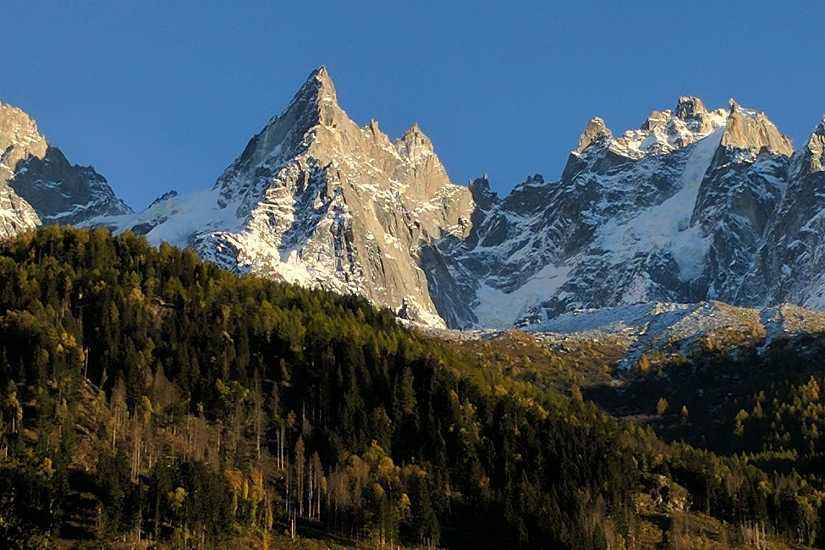
\includegraphics[width=0.2\textwidth]{mountain}
	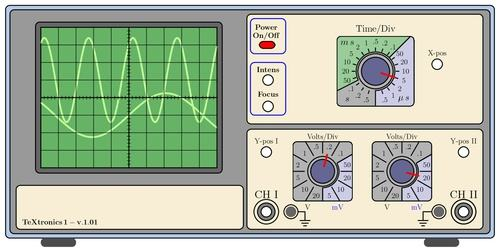
\includegraphics[width=0.2\textwidth]{oscilloscope}
	
	
	
\includegraphics[angle=-45,width=0.2\textwidth]{lion}
	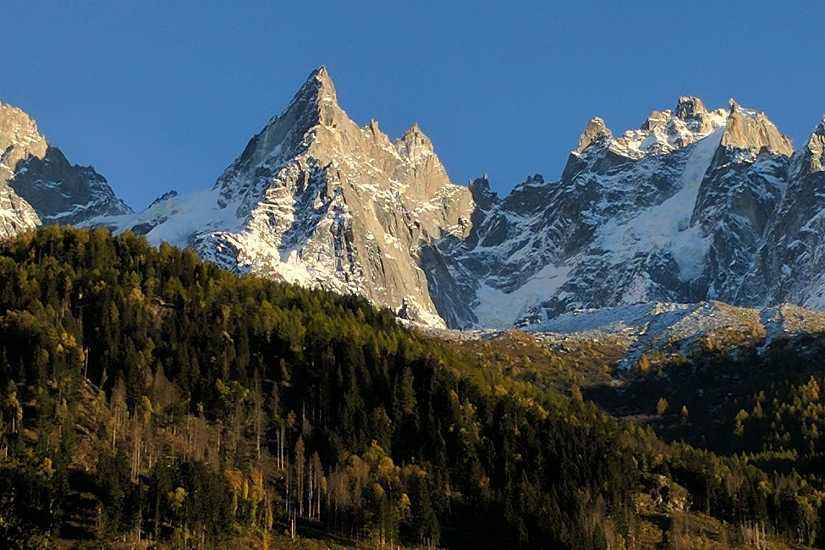
\includegraphics[width=0.2\textwidth]{mountain}
	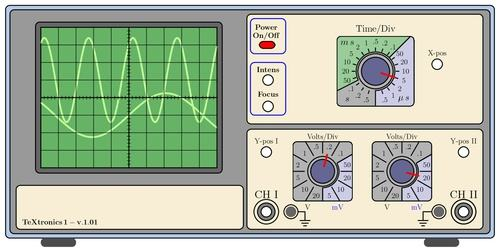
\includegraphics[angle=45,width=0.2\textwidth]{oscilloscope}
\end{document}
